\documentclass{beamer}
\usepackage{ucs}
\usepackage[utf8x]{inputenc}
\usepackage[T1]{fontenc}

\usepackage{graphicx}
\usepackage{tipa}

\begin{document}
\title{Pedagogiske program og språkteknologi \\ jkhjkhkhjk.}   
\author{Lene Antonsen\\ \begin{figure}  \scalebox{0.10}[0.10]{
\includegraphics{img/LogoSamisk}} \end{figure}} 
\date{} 


\frame{\titlepage} 

%\frame{\frametitle{Table of contents}\tableofcontents} 


%\section{Section no.1} 

\frame{\frametitle{ }
\begin{block}{ }
\textit{http://giellatekno.uit.no/oahpa/}\\
\end{block}{ }
Sametinget og Universitetet i Tromsø har finansiert prosjektet
\begin{block}{ }
Lene Antonsen, Biret Ánne Bals Baal, \\ Saara Huhmarniemi, Trond Trosterud
\end{block}{ }
}


\frame{\frametitle{VISL-programmene}
\begin{block}{ }
\textbf{Lære grammatikk:}\\
\end{block}{ }
Ordklasser, syntaks.\\

Syd-dansk Universitet lea ráhkadan teknologiija. \\
Mii leat lasihan analyserejuvvon sámegiel cealkagiid.
}

\frame{\frametitle{ }
\scalebox{.43}[.43]{\includegraphics{img/shooting3.png}}
}
\frame{\frametitle{ }
\scalebox{.45}[.45]{\includegraphics{img/Cealkkamuorra3.png}}
}
\frame{\frametitle{ }\scalebox{.44}[.5]{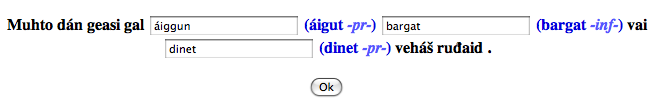
\includegraphics{img/killerquest.png}}
}
\frame{\frametitle{ }\scalebox{.5}[.5]{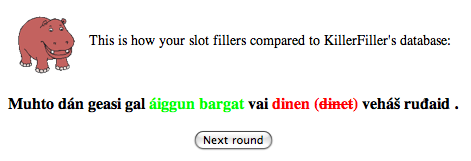
\includegraphics{img/killeransw.png}}
}

\frame{\frametitle{OAHPA-programmene}
\begin{block}{ }
\textbf{Lære samisk:}\\
\end{block}{}
\begin{itemize}
\item \textbf{Leksa}: Sátnequiz - samisk/norsk og norsk/samisk
\item  \textbf{Numra}: Trene på tall
\item  \textbf{Morfa}: Trene på å bøye ord, også i setninger
\item  \textbf{Vasta}: Trene på å svare på spørsmål
\item  \textbf{Sahka}: Delta i dialog om et tema
\end{itemize}
}

\frame{\frametitle{Pedagogiske programmer}

Det er vanligvis ikke spåkteknologi i pedagogiske programmer, men
\begin{itemize}
\item multiple choice 
\item stringmatch, f.eks. \textit{viesus} = 6 merker: v i e s u s
\end{itemize} \pause
\begin{block}{ }
Spåkteknologi:
\begin{itemize}
\item analyse, f.eks. \textit{viesus} = \textit{viessu} N Sg Loc
\end{itemize}
\end{block}{ }
}


\frame{\frametitle{CALL og ICALL} 
CALL \\
ICALL
}


\frame{\frametitle{Vår visjon} 
Programmet skal veilede brukeren på samme måte som en lærer gjør.
}

\frame{\frametitle{Vasta -- Trene på å svare på spørsmål} 
\scalebox{0.90}[0.90]{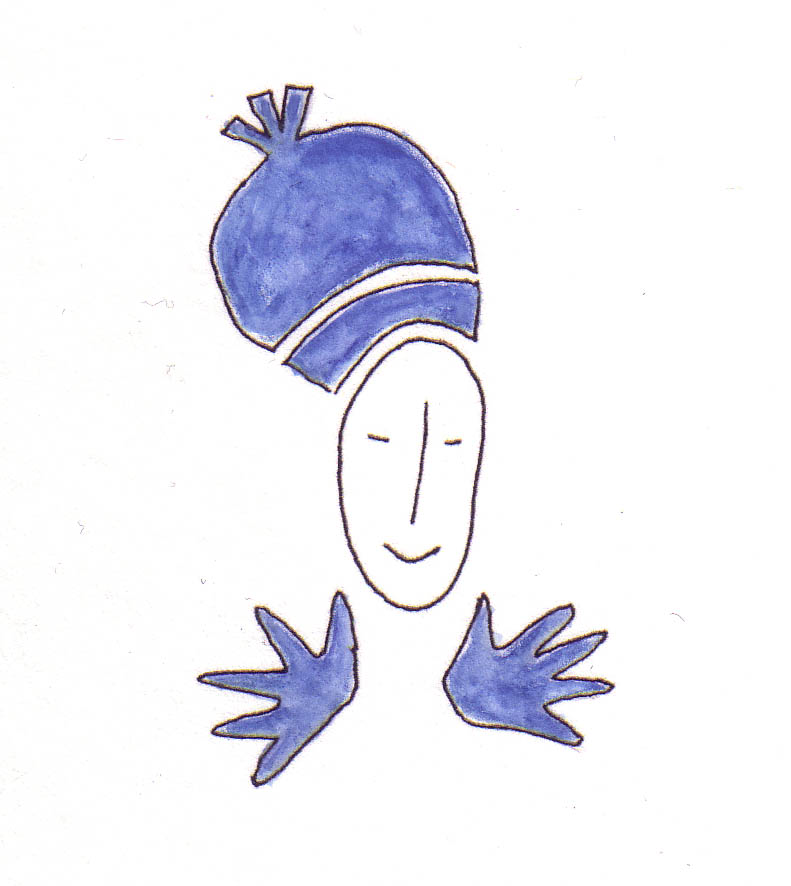
\includegraphics{img/vasta.png}} \\
}

\frame{\frametitle{Vasta} 
\scalebox{0.35}[0.35]{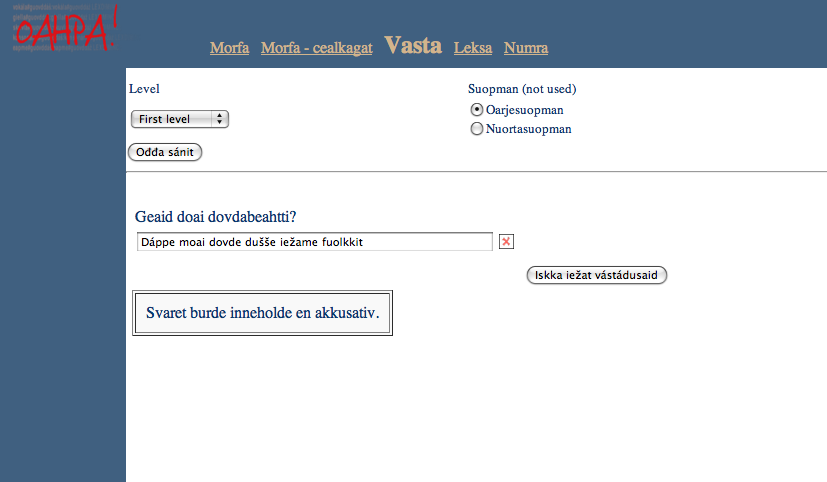
\includegraphics{img/vasta_jear.png}}
}


\frame{\frametitle{Maid don lohket ikte?} 

Akseptable svar:
\begin{itemize}
\item Mun han lohken ollu áviissaid. 
\item Ikte mun gal lohken buori girjji. 
\item In lohkan maidege. 
\item Ikte in lohkan.
\end{itemize}
}

\frame{\frametitle{Maid don lohket ikte?} 

Vasta-programmet veileder på svaret ikke er akseptabelt:
\begin{itemize}
\item Mun lohket ollu áviissaid. \\ $\rightarrow$ Husk kongruens mellom subjekt og verbal.  
\item Mun lohken ollu áviissat. \\ $\rightarrow$ Objektet skal være i akkusativ. 
\item Don lohket ollu áviissaid. \\ $\rightarrow$ Er du sikker på at du svarer i riktig person?  
\end{itemize}
}

\frame{\frametitle{Vårt system} 
\scalebox{0.65}[0.65]{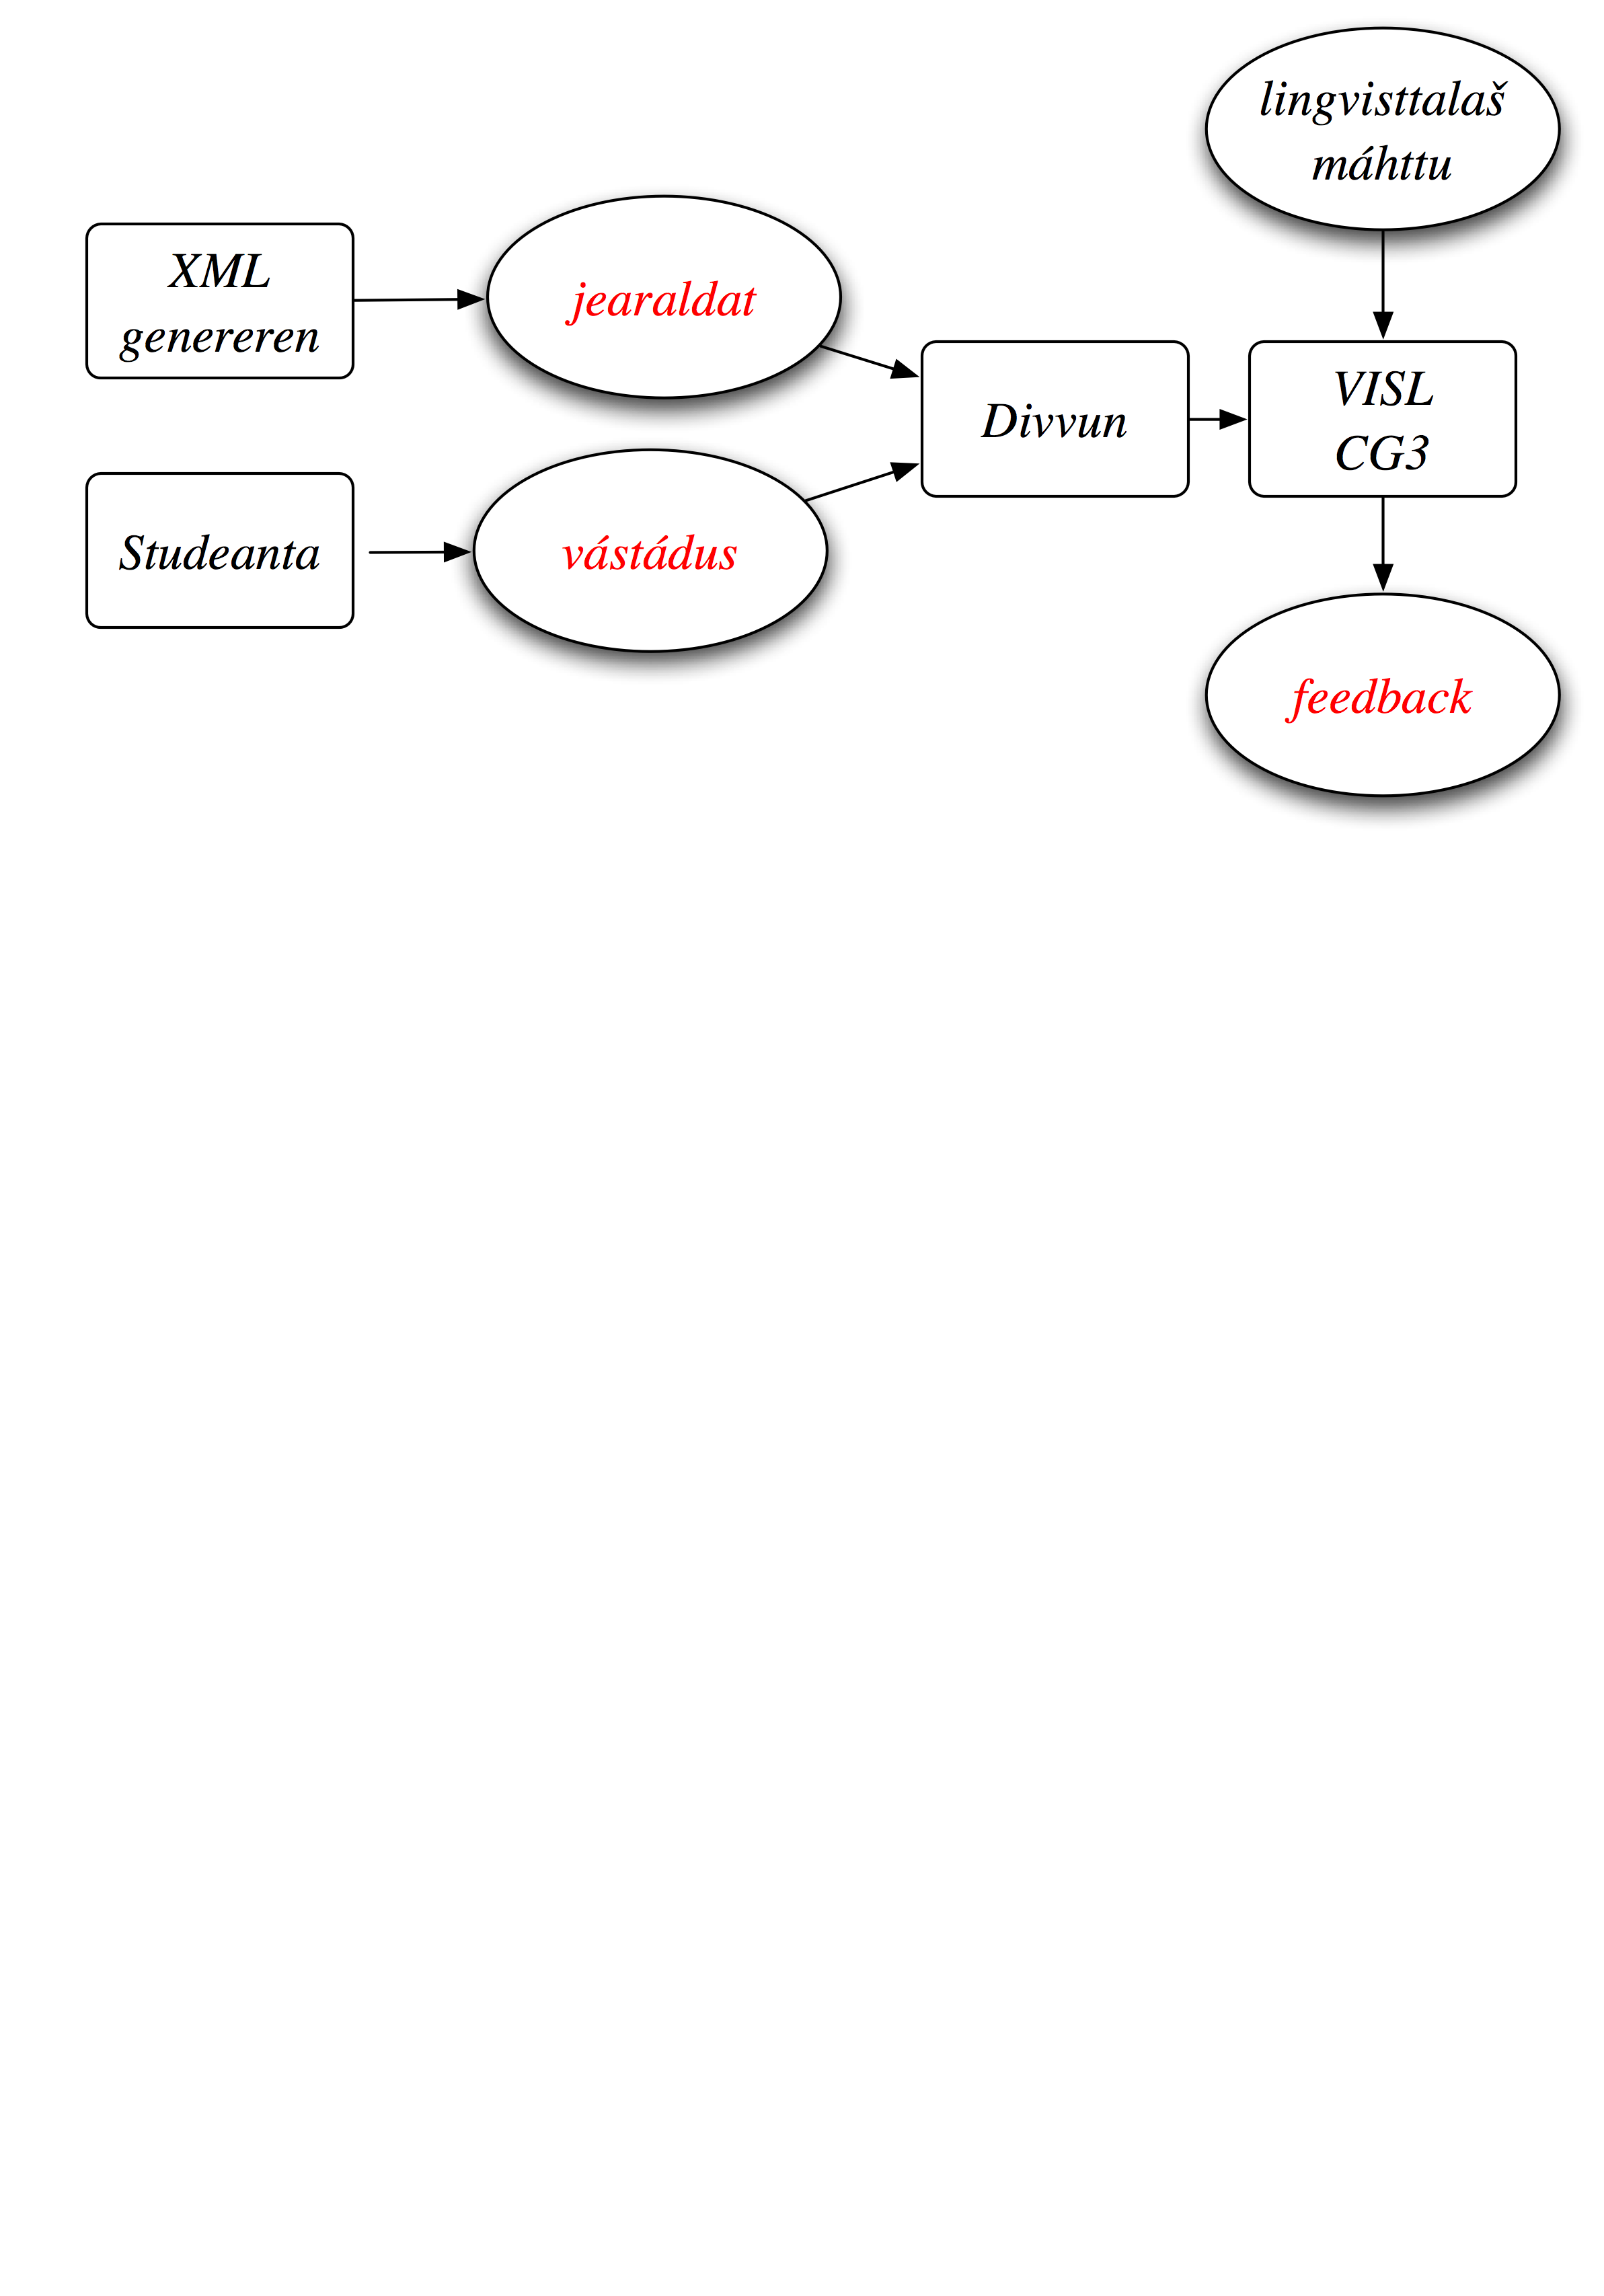
\includegraphics{img/skovi.png}} 
} 


\frame{\frametitle{Generere spørsmål} 
      <text>Maid SUBJ MAINV ikte</text>
}

\frame{\frametitle{Kunnskap i lingvistikk} 
Vi bruker vår kunnskap om:
\begin{itemize}
\item samisk syntaks	
\item elevenes mellomspråk
\end{itemize}
}


\frame{\frametitle{Naturlig dialog?}
\begin{block}{ }
\textbf{Didaktikk versus pragmatikk} \\
\end{block}{ }
Vi ønsker at brukeren skal trene på alle personer og tall. Derfor:
\begin{itemize}
\item{Svaret må inneholde finitt verb}
\item{Man må svare med samme verb når det er naturlig å gjøre det}
\item{Ikke inkluderende 1. p dualis og pluralis }
\item{\textit{Jeg-vet-ikke} aksepteres ikke som svar}
\end{itemize}
}



\frame{\frametitle{Rette eller ikke?}
\begin{block}{ }
\textbf{Det er bedre at ikke alt blir rettet, enn å rette det som er riktig}
\end{block}{ }
- men er brukeren fornøyd med det?

}

\frame{\frametitle{Evalueren ja buorideapmi}
\begin{itemize}
\item Responsa geavaheddjiin
\item Responsa oahpaheddjiin
\item Ráhkadit vástáduskorpusa (Vasta-log interneahtas)
\end{itemize}
}



%\subsection{Lists II}
%\frame{\frametitle{numbered lists}
%\begin{enumerate}
%\item Introduction to  \LaTeX  
%\item Course 2 
%\item Termpapers and presentations with \LaTeX 
%\item Beamer class
%\end{enumerate}
%}
%\frame{\frametitle{numbered lists with pause}
%\begin{enumerate}
%\item Introduction to  \LaTeX \pause 
%\item Course 2 \pause 
%\item Termpapers and presentations with \LaTeX \pause 
%\item Beamer class
%\end{enumerate}
%}
%
%\section{Section no.3} 
%\subsection{Tables}
%\frame{\frametitle{Tables}
%\begin{tabular}{|c|c|c|}
%\hline
%\textbf{Date} & \textbf{Instructor} & \textbf{Title} \\
%\hline
%WS 04/05 & Sascha Frank & First steps with  \LaTeX  \\
%\hline
%SS 05 & Sascha Frank & \LaTeX \ Course serial \\
%\hline
%\end{tabular}}
%
%
%\frame{\frametitle{Tables with pause}
%\begin{tabular}{c c c}
%A & B & C \\ 
%\pause 
%1 & 2 & 3 \\  
%\pause 
%A & B & C \\ 
%\end{tabular} }
%
%
%\section{Section no. 4}
%\subsection{blocs}
%\frame{\frametitle{blocs}
%
%\begin{block}{title of the bloc}
%bloc text
%\end{block}
%
%\begin{exampleblock}{title of the bloc}
%bloc text
%\end{exampleblock}
%
%
%\begin{alertblock}{title of the bloc}
%bloc text
%\end{alertblock}
\end{document}

